\section{Metodologia}

O desenvolvimento de fontes de alimentação lineares exige o entendimento aprofundado de diversos componentes eletrônicos e seus papéis no circuito. Nesta seção, abordamos os conceitos teóricos que embasam o projeto, destacando os principais elementos utilizados e suas aplicações práticas.

O projeto solicitado consiste em uma fonte de alimentação linear com realimentação de tensão, capaz de fornecer uma tensão ajustável entre 3 e 15 V, com corrente máxima de 1 A. O circuito deve incluir limitação automática de corrente, proteção contra curto-circuito e monitoramento de tensão, indicando as condições de operação.

Dessa maneira, a fim de atender às especificações, o projeto foi dividido em três etapas principais: a implementação do regulador de tensão, a proteção contra sobrecorrente e a sinalização de tensão.

\subsection{Especificações do Projeto}

O projeto foi desenvolvido com base nas seguintes especificações:

\begin{itemize}
    \item Tensão de saída ajustável entre \textbf{2,4 V e 18 V};
    \item Corrente máxima de \textbf{2 A};
    \item Limitação automática de corrente configurada para \textbf{1,3 A};
    \item Sinalização de sobrecorrente por LED indicador;
    \item Monitoramento de tensão com sinalização por janela:
    \begin{itemize}
        \item \textbf{LED verde}: Tensão menor que \textbf{6 V};
        \item \textbf{LED amarelo}: Tensão entre \textbf{6 V e 10 V};
        \item \textbf{LED vermelho}: Tensão maior que \textbf{10 V}.
    \end{itemize}
\end{itemize}

\subsection{Dimensionamento dos Componentes}

\subsubsection{Regulador de Tensão}

O regulador de tensão é o componente central da fonte de alimentação, responsável por manter a tensão de saída constante, independentemente das variações na carga ou na tensão de entrada. O circuito é composto por quatro elementos principais: o elemento de passagem, o gerador de corrente constante (GCC), o amplificador de erro.

\subsubsection*{Elemento de Passagem}

Esse componente é responsável por fornecer a corrente necessária para a carga, ajustando-a conforme a tensão de saída. Sendo assim, o elemento de passagem deve ser capaz de suportar a corrente máxima exigida pela carga e a faixa de tensão de operação.

Dessa forma, os requisitos para o elemento de passagem são:

\begin{itemize}
    \item Tensão de entrada: 24 V;
    \item Tensão de saída máxima: 18 V;
    \item Tensão de saída mínima: 0 V (curto-circuito);
    \item Corrente máxima: 2 A.
\end{itemize}

A partir desses requisitos, podemos calcular a potência máxima dissipada pelo elemento de passagem, a corrente de base necessária e a queda de tensão entre coletor e emissor.

\subsubsection*{Cálculo da potência máxima dissipada}  
A potência dissipada pelo elemento de passagem ocorre quando a diferença entre a tensão de entrada e a tensão de saída é máxima e a corrente fornecida à carga é máxima.  

\[
P_{diss} = (V_{in} - V_{out}) \cdot I_{load}
\]

Substituindo os valores extremos:  
\[
P_{diss\_max} = (24\,V - 0\,V) \cdot 2\,A = 48\,W
\]

Portanto, o elemento de passagem deve ser montado em um dissipador de calor capaz de suportar pelo menos 48 W de dissipação para evitar superaquecimento.  

Dessa forma, a fonte de entrada deve fornecer pelo menos 18,7 V para garantir a regulação adequada da saída.  

\subsubsection*{Escolha do componente}  
Com base nos cálculos realizados, foi escolhido o transistor Darlington TIP142, que atende aos seguintes requisitos:  
\begin{itemize}
    \item Corrente máxima de coletor: 10 A;
    \item Potência máxima dissipada: 125 W;
    \item Ganho de corrente (\(\beta\)): 1000 (típico);
    \item Tensão máxima coletor-emissor: 100 V.
\end{itemize}

O uso do TIP142, sendo um transistor Darlington, oferece uma vantagem significativa em termos de ganho de corrente (\(\beta\)), reduzindo a corrente necessária na base para cerca de:  
\[
I_B = \frac{I_C}{\beta} = \frac{2\,A}{1000} = 2\,mA
\]

Essa característica simplifica o circuito de controle e reduz a potência exigida na etapa de acionamento. Além disso, o TIP142 suporta margens amplas de potência e tensão, tornando-o adequado para este projeto.  

\subsubsection{Gerador de Corrente Constante (GCC)}  

O gerador de corrente constante (GCC) é um elemento indispensável no regulador de tensão, sendo responsável por fornecer uma corrente estável à base do transistor de potência. Ele é constituído por um transistor PNP, um diodo Zener e resistores de polarização, garantindo o funcionamento confiável e preciso do circuito.  

A corrente constante gerada pelo GCC é determinada pela tensão sobre o diodo Zener (\(V_Z\)) e a resistência conectada ao emissor (\(R_E\)), ajustando-se para compensar a queda de tensão base-emissor (\(V_{BE}\)) do transistor. A fórmula que rege esse comportamento é:  

\[
I_C = \frac{V_Z - V_{BE}}{R_E}
\]

Onde:  
\begin{itemize}
    \item \(I_C\): corrente de saída do GCC;
    \item \(V_Z\): tensão estabilizada pelo diodo Zener;
    \item \(V_{BE}\): queda de tensão base-emissor;
    \item \(R_E\): resistor de limitação de corrente.
\end{itemize}  

\subsubsection*{Diodo Zener}

Para o projeto, foi escolhido o diodo Zener 1N4733, com \(V_Z = 5,1 \, \text{V}\) e potência de \(1 \, \text{W}\).

\subsubsection*{Resistor de polarização}

A fim de termos na base do transistor uma corrente mínima de 2 mA, foi definido um valor de \(20 \, \text{mA}\) para a corrente de coletor. Assim, o resistor de polarização (\(R_E\)) é calculado como:

\[
R_E = \frac{V_Z - V_{BE}}{I_C} = \frac{5,1 \, \text{V} - 0,7 \, \text{V}}{20 \times 10^{-3} \, \text{A}} = 220 \, \Omega
\]

\[
P_{R_E} = V_{R_E}^2 / R_E = (5,1 \, \text{V} - 0,7 \, \text{V})^2 / 220 \, \Omega = 88 \, \text{mW}
\]

Assim, um resistor comercial de \(220 \, \Omega\) com potência mínima de \(0,25 \, \text{W}\) foi selecionado, garantindo segurança térmica.  

\subsubsection*{Cálculo de \(R_Z\)}  

Para a devida polarização do diodo Zener, calcularemos o valor de \(R_Z\) a fim de obtermos uma corrente de 10\% da corrente máxima do Zener (\(I_{Z_max}\)).

\[
I_{R_Z} = (P_Z / V_Z = 1 \, \text{W} / 5,1) * 10\% = 19,6 \, \text{mA}
\]

A tensão no resistor \(R_Z\) é a diferença entre a tensão de alimentação (\(V_{CC}\)) e a tensão do Zener (\(V_Z\)):  

\[
V_{R_Z} = V_{CC} - V_Z = 24 \, \text{V} - 5,1 \, \text{V} = 18,9 \, \text{V}
\]

Com isso, o valor de \(R_Z\) é calculado:  

\[
R_Z = \frac{V_{R_Z}}{I_{R_Z}} = \frac{18,9 \, \text{V}}{21 \times 10^{-3} \, \text{A}} \approx 900 \, \Omega
\]

\[
P_{R_Z} = \frac{V_{R_Z}^2}{R_E} = \frac{18,9 \, \text{V}^2}{820 \, \Omega} = 435 \, \text{mW}
\]

Selecionamos um resistor comercial de \(820 \, \Omega\) e potência mínima de \(0,5 \, \text{W}\) para garantir a segurança térmica.

\subsubsection*{Transistor PNP}  

O transistor 2N3906 foi escolhido como o PNP para o GCC devido às suas características:  

\begin{itemize}
    \item Corrente máxima do coletor (\(I_{C(max)}\)): \(200 \, \text{mA}\);
    \item Potência máxima dissipada: \(625 \, \text{mW}\);
    \item Ganho de corrente (\(h_{FE}\)): \(100\) (mínimo para \(I_C = 10 \, \text{mA}\));
    \item Tensão máxima coletor-emissor (\(V_{CE(max)}\)): \(40 \, \text{V}\).
\end{itemize}  

\subsubsection*{Conclusão do GCC}  

Com os cálculos apresentados, os componentes do GCC foram dimensionados conforme:  
\begin{itemize}
    \item Diodo Zener: 1N4733 (\(5,1 \, \text{V}\));
    \item Resistor de polarização: \(820 \, \Omega, \, 0,5 \, \text{W}\);
    \item Transistor PNP: 2N3906.
    \item Resistor limitador de corrente: \(220 \, \Omega, \, 0,25 \, \text{W}\).
\end{itemize}

Esse dimensionamento assegura que o GCC forneça uma corrente constante de \(20 \, \text{mA}\) de forma confiável, atendendo às demandas do regulador de tensão.  

\subsubsection{Amplificador de Erro}

O amplificador de erro é responsável por ajustar a corrente na base do transistor de potência, controlando assim a corrente que flui para a carga. Ele é composto por um transistor NPN, uma tensão de referência e um divisor de tensão, garantindo a estabilidade e a precisão do circuito.

\subsubsection*{Tensão de referência}

Em virtude da necessidade de ajuste da tensão de saída entre 2,4 V e 18 V, não foi possível utilizar um diodo Zener convencional como referência. Portanto, optou-se pelo uso de dois diodos convencionais em série, que fornecem uma tensão de referência de aproximadamente 1,4 V.

Para garantir a tensão de referência estável, foram escolhidos diodos 1N4007 devido à sua ampla faixa de operação e baixo custo e especificações de tensão reversa de 1000 V e corrente média de 1 A.

Sendo assim, foi adicionado um resistor de polarização ligado aos diodos para garantir a corrente mínima necessária para a estabilidade da tensão de referência.

Segundo o datasheet do 1N4007, a corrente máxima de pico é de 30 A, e a corrente média é de 1 A. Portanto, o resistor de polarização foi calculado para fornecer uma corrente de 20 mA, garantindo a estabilidade da tensão de referência.

\[
R_D = \frac{V_{CC} - V_{D}}{I_{D}} = \frac{24 \, \text{V} - 1,4 \, \text{V}}{20 \, \text{mA}} = 1k13 \, \Omega
\]

\[
P_{R_D} = \frac{V_{R_D}^2}{R_D} = \frac{22,6 \, \text{V}^2}{1k2 \, \Omega} = 426 \, \text{mW}
\]

Portanto, um resistor comercial de \(1k2 \, \Omega\) e potência mínima de \(0,5 \, \text{W}\) foi selecionado para garantir a segurança térmica.

\subsubsection*{Divisor de tensão}

A partir da tensão de referência, temos que a tensão na base do transistor NPN é:

\[
V_B = V_{Z} + V_{BE} = 1,4 \, \text{V} + 0,7 \, \text{V} = 2,1 \, \text{V}
\]

Sendo assim, para garantir uma tensão de saída mínima dentro do intervalo especificado, utilizamos um divisor de tensão compostor por um potenciômetro de 2 k\(\Omega\) e um resistor de 220 \(\Omega\). Dessa forma, a tensão de saída é:

\[
V_{\text{out\_min}} = \frac{V_B}{R_1 + R_{\text{pot}}} \times R_{\text{total}}
\]

\[
V_{\text{out\_min}} = \frac{2,1 \, \text{V}}{220 \, \Omega + 2000 \, \Omega} \times 2220 \, \Omega
\]

\[
V_{\text{out\_min}} = 2,1 \, \text{V}
\]

Dessa mesma forma, a tensão de saída máxima é:

\[
V_{\text{out\_max}} = \frac{V_B}{R_1} \times R_{\text{total}}
\]

\[
V_{\text{out\_min}} = \frac{2,1 \, \text{V}}{220 \, \Omega} \times 2220 \, \Omega
\]

\[
V_{\text{out\_min}} = 21,19 \, \text{V}
\]

\subsubsection*{Transistor NPN}

O transistor NPN utilizado no amplificador de erro é o 2N2222, que atende aos seguintes requisitos:

\begin{itemize}
    \item Corrente máxima do coletor (\(I_{C(max)}\)): \(800 \, \text{mA}\);
    \item Potência máxima dissipada: \(500 \, \text{mW}\);
    \item Ganho de corrente (\(h_{FE}\)): \(150\);
    \item Tensão máxima coletor-emissor (\(V_{CE(max)}\)): \(40 \, \text{V}\).
\end{itemize}

\subsubsection*{Conclusão do amplificador de erro}

Com os cálculos apresentados, os componentes do amplificador de erro foram dimensionados conforme:

\begin{itemize}
    \item Tensão de referência: 2 diodos 1N4007 em série (\(1,4 \, \text{V}\));
    \item Divisor de tensão: potenciômetro de 2 k\(\Omega\) e resistor de 220 \(\Omega\);
    \item Transistor NPN: 2N2222.
\end{itemize}

\subsubsection*{Circuito final do regulador de tensão}

O circuito final do regulador de tensão é composto pelos elementos de passagem, gerador de corrente constante e amplificador de erro, conforme a figura a seguir:

\begin{figure}[H]
    \centering
    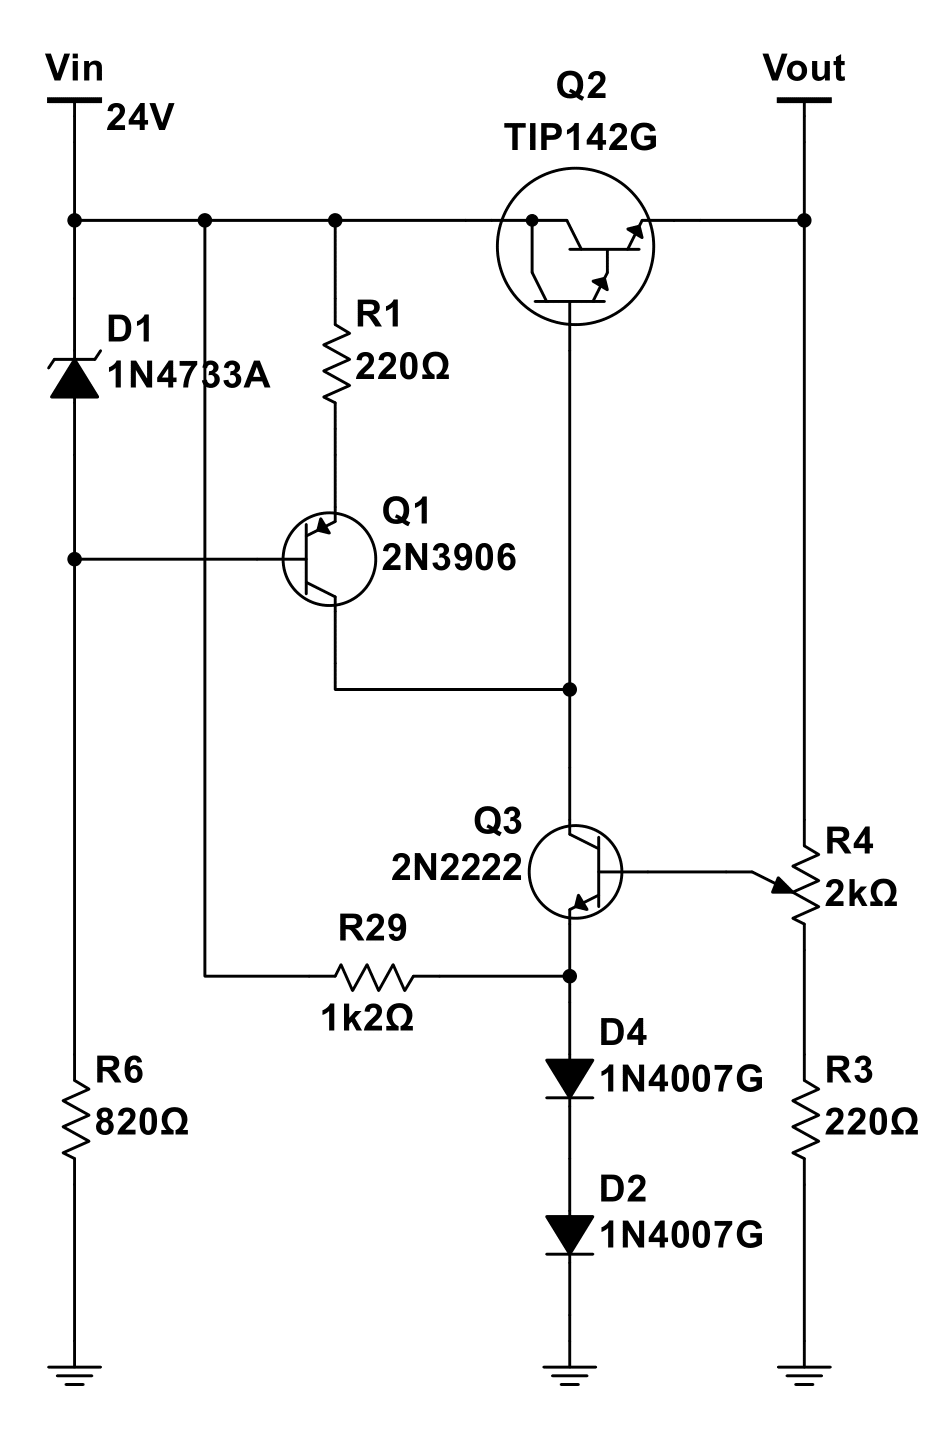
\includegraphics[width=0.6\textwidth]{../imagens/circuito_regulador.png}
    \caption{Circuito final do regulador de tensão}
    \label{fig:regulador_tensao}
\end{figure}

\subsubsection{Limitador de corrente e proteção contra curto-circuito}

A proteção contra surtos de corrente é essencial para garantir a segurança do circuito e dos dispositivos conectados. Para isso, foi implementado um circuito de limitação de corrente e proteção contra curto-circuito unidos em um único bloco. Onde, caso a corrente de saída ultrapasse o limite de 1,3 A, o circuito entra em ação, roubando a corrente excedente e protegendo o circuito de danos.

\subsubsection*{Limitador de corrente}

O limitador de corrente é composto por um transistor PNP e um resistor de limitação de corrente ligado entre a base e o emissor. O transistor é acionado quando a corrente de saída ultrapassa o limite de 1,3 A, desviando o excesso de corrente que seria fornecida a base do transistor de potência.

Dessa forma, podemos calcular o valor do resistor de limitação de corrente para garantir que o transistor PNP entre em saturação quando a corrente de saída atingir 1,3 A.


\[
R_{SC} = \frac{V_{BE}}{I_{o\_max}} = \frac{0,7 \, \text{V}}{1,3 \, \text{A}} = 0,538 \, \Omega
\]

Para garantir uma corrente mínima de 1,3 A, foi escolhido o valor comercial de \(0,47 \, \Omega\).

\[
P_{R_{SC}} = \frac{V_{BE}^2}{R_{SC}} = \frac{(0,7 \, \text{V})^2}{0,47 \, \Omega} = 1,04 \, \text{W}
\]

Em virtude disso, um resistor de \(0,47 \, \Omega\) e potência mínima de \(2 \, \text{W}\) foi selecionado para garantir a segurança térmica.

Sendo assim, agora devemos calcular a nova corrente de saída máxima, considerando a definição do resistor limitador de corrente.

\[
I_{o\_max} = \frac{V_{BE}}{R_{SC}} = \frac{0,7 \, \text{V}}{0,47 \, \Omega} = 1,49 \, \text{A}
\]

\subsubsection*{Sinalização de sobrecorrente}

Para sinalizar a ocorrência de sobrecorrente, foi adicionado um outro transistor PNP, com seus terminais de base e emissor ligados ao circuito de limitação de corrente e o coletor conectado a um LED indicador. Dessa forma, quando a corrente de saída ultrapassar 1,3 A, o transistor PNP entra em saturação, acionando o LED indicador.

Para correta operação do LED, foi adicionado um resistor limitador de corrente em série, garantindo o pleno funcionamento do LED e a segurança do circuito.

\[
R_{LED} = \frac{V_{CC} - V_{LED}}{I_{LED}} = \frac{24 \, \text{V} - 2 \, \text{V}}{20 \, \text{mA}} = 1k \, \Omega
\]

\[
P_{R_{LED}} = \frac{V_{R_{LED}}^2}{R_{LED}} = \frac{22 \, \text{V}^2}{1k \, \Omega} = 484 \, \text{mW}
\]

Portanto, um resistor de \(1k \, \Omega\) e potência mínima de \(0,5 \, \text{W}\) foi selecionado para garantir a segurança térmica.

\subsubsection*{Conclusão do limitador de corrente}

Com os cálculos apresentados, os componentes do limitador de corrente e proteção contra curto-circuito foram dimensionados conforme:

\begin{itemize}
    \item Resistor de limitação de corrente: \(0,47 \, \Omega, \, 2 \, \text{W}\);
    \item Transistor PNP de sinalização: 2N2222;
    \item Transistor PNP de limitação de corrente: 2N2222;
    \item Resistor de sinalização: \(1k \, \Omega, \, 0,5 \, \text{W}\).
\end{itemize}

Dessa forma, o circuito de limitação de corrente e proteção contra curto-circuito foi implementado com sucesso, garantindo a segurança do circuito e dos dispositivos conectados.

\subsubsection*{Circuito final do limitador de corrente}

O circuito final do limitador de corrente e proteção contra curto-circuito é composto pelos elementos de limitação de corrente, sinalização de sobrecorrente e proteção contra curto-circuito, conforme a figura a seguir:

\begin{figure}[H]
    \centering
    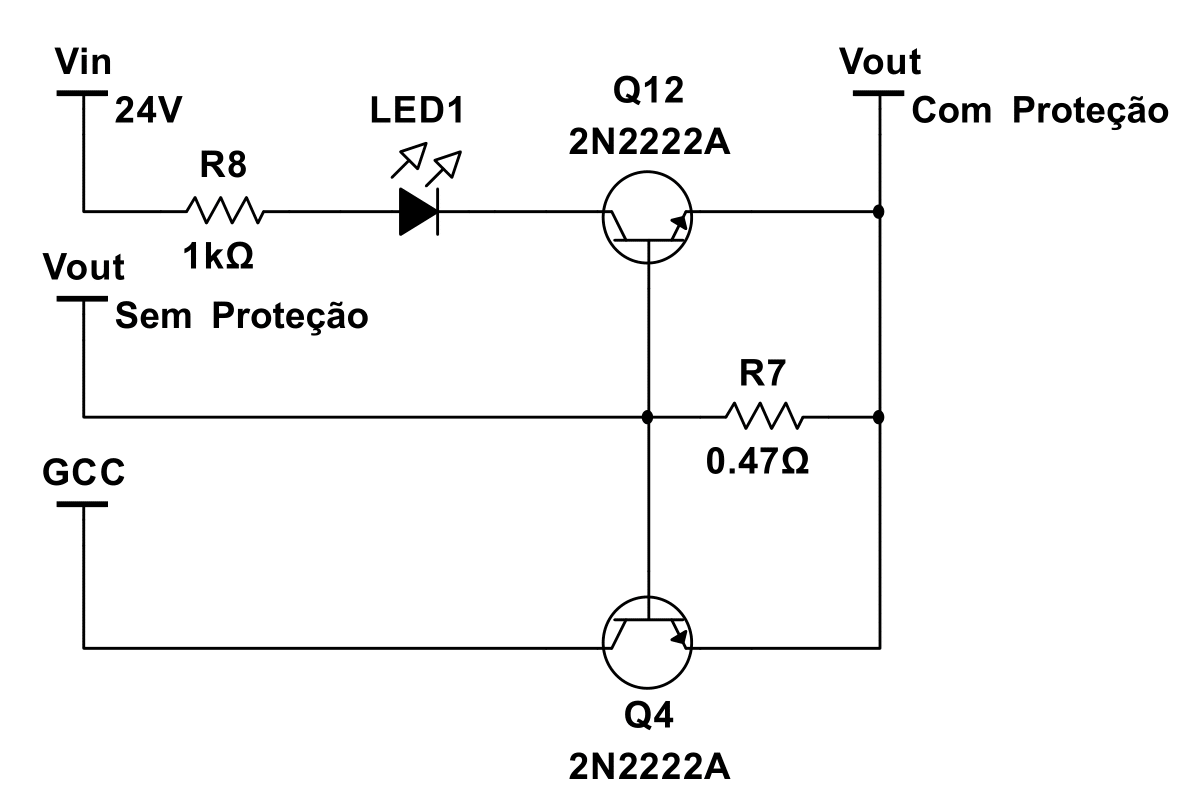
\includegraphics[width=0.6\textwidth]{../imagens/circuito_protecao.png}
    \caption{Circuito final do limitador de corrente}
    \label{fig:protecao}
\end{figure}

\subsubsection{Monitor de Tensão}

O monitor de tensão é responsável por indicar a tensão de saída do regulador de tensão, sinalizando ao usuário as condições de operação do circuito. Para isso, foram implementados LEDs indicadores de três cores, que acendem conforme a tensão de saída atinge determinados valores.

\begin{itemize}
    \item LED verde: tensão menor que 6 V;
    \item LED amarelo: tensão entre 6 V e 10 V;
    \item LED vermelho: tensão maior que 10 V.
\end{itemize}

Dessa forma, o monitor de tensão foi implementado seguindo o conceito de lógica digital, onde cada LED é acionado conforma uma combinação de tensões de referência e a tensão de saída do regulador.

Para isso, é necessário criar um circuito que compare a tensão de saída com as tensões de referência e gere níveis lógicos para acionar os LEDs indicadores.

\subsubsection*{Comparador de tensão}

Como o trabalho deve ser realizado apenas com componentes discretos, o uso de um amplificador operacional não é permitido. Portanto, foi implementado um comparador de tensão utilizando transistores NPN e PNP, que geram níveis lógicos conforme a tensão de saída do regulador.

Sendo assim, foi criado um circuito com um transistor NPN que em sua base está um diodo Zener para gerar uma tensão de referência, um divisor de tensão com trimpot em sua base para ajustar a tensão de referência e um transistor PNP que é acionado conforme a tensão de saída ultrapassa a tensão de referência. Resultando em 0 V na saída do transistor PNP quando a tensão de saída é menor que a tensão de referência e 24 V quando a tensão de saída é maior que a tensão de referência.

Foram utilizados diodos Zener 1N4733 para gerar a tensão de referência de 6 V e 1N4739 para gerar a tensão de referência de 10 V. Além disso, foi utilizado um trimpot de 100 k\(\Omega\) em série com um resistor de 1 k\(\Omega\) para ajustar a tensão de referência.

Como já foi calculador anteriormente o resistor de polarização do diodo Zener 1N4733, devemos apenas calcular o resistor de polarização do diodo Zener 1N4739.

Para a devida polarização do diodo Zener, calcularemos o valor de \(R_Z\) a fim de obtermos uma corrente de 10\% da corrente máxima do Zener (\(I_{Z_max}\)).

\[
I_{R_Z} = (P_Z / V_Z = 1 \, \text{W} / 9,1) * 10\% = 10,9 \, \text{mA}
\]

A tensão no resistor \(R_Z\) é a diferença entre a tensão de alimentação (\(V_{CC}\)) e a tensão do Zener (\(V_Z\)):  

\[
V_{R_Z} = V_{CC} - V_Z = 24 \, \text{V} - 5,1 \, \text{V} = 14,9 \, \text{V}
\]

Com isso, o valor de \(R_Z\) é calculado:  

\[
R_Z = \frac{V_{R_Z}}{I_{R_Z}} = \frac{4,9 \, \text{V}}{10,9 \times 10^{-3} \, \text{A}} \approx 1355 \, \Omega
\]

\[
P_{R_Z} = \frac{V_{R_Z}^2}{R_E} = \frac{4,9 \, \text{V}^2}{1200 \, \Omega} = 185 \, \text{mW}
\]

Selecionamos um resistor comercial de \(1k2 \, \Omega\) e potência mínima de \(0,5 \, \text{W}\) para garantir a segurança térmica.

\subsubsection*{Conclusão do comparador de tensão}

Com os cálculos apresentados, os componentes do comparador de tensão foram dimensionados conforme:

\begin{itemize}
    \item Diodo Zener 1N4733: \( 5,1 \, \text{V} \);
    \item Diodo Zener 1N4739: \( 9,1 \, \text{V} \);
    \item Trimpot: \( 100 \, \text{k}\Omega \);
    \item Resistor do trimpot: \( 1 \, \text{k}\Omega \);
    \item Resistor de polarização do diodo Zener 1N4739: \( 1{,}2 \, \Omega, \, 0{,}5 \, \text{W} \);
    \item Resistor de polarização do diodo Zener 1N4733: \( 820 \, \Omega, \, 0{,}5 \, \text{W} \);
    \item Transistor NPN: 2N2222;
    \item Transistor PNP: 2N3906;
    \item Resistores de polarização: \( 10 \, \text{k}\Omega, \, 0{,}25 \, \text{W} \).
\end{itemize}

\subsubsection*{Circuito final do comparador de tensão}

O circuito final do comparador de tensão é composto pelos elementos de comparação, tensão de referência e sinalização, alterando apenas o diodo Zener 1N4739 para 9,1 V e seu resistor de polarização, conforme a figura a seguir:

\begin{figure}[H]
    \centering
    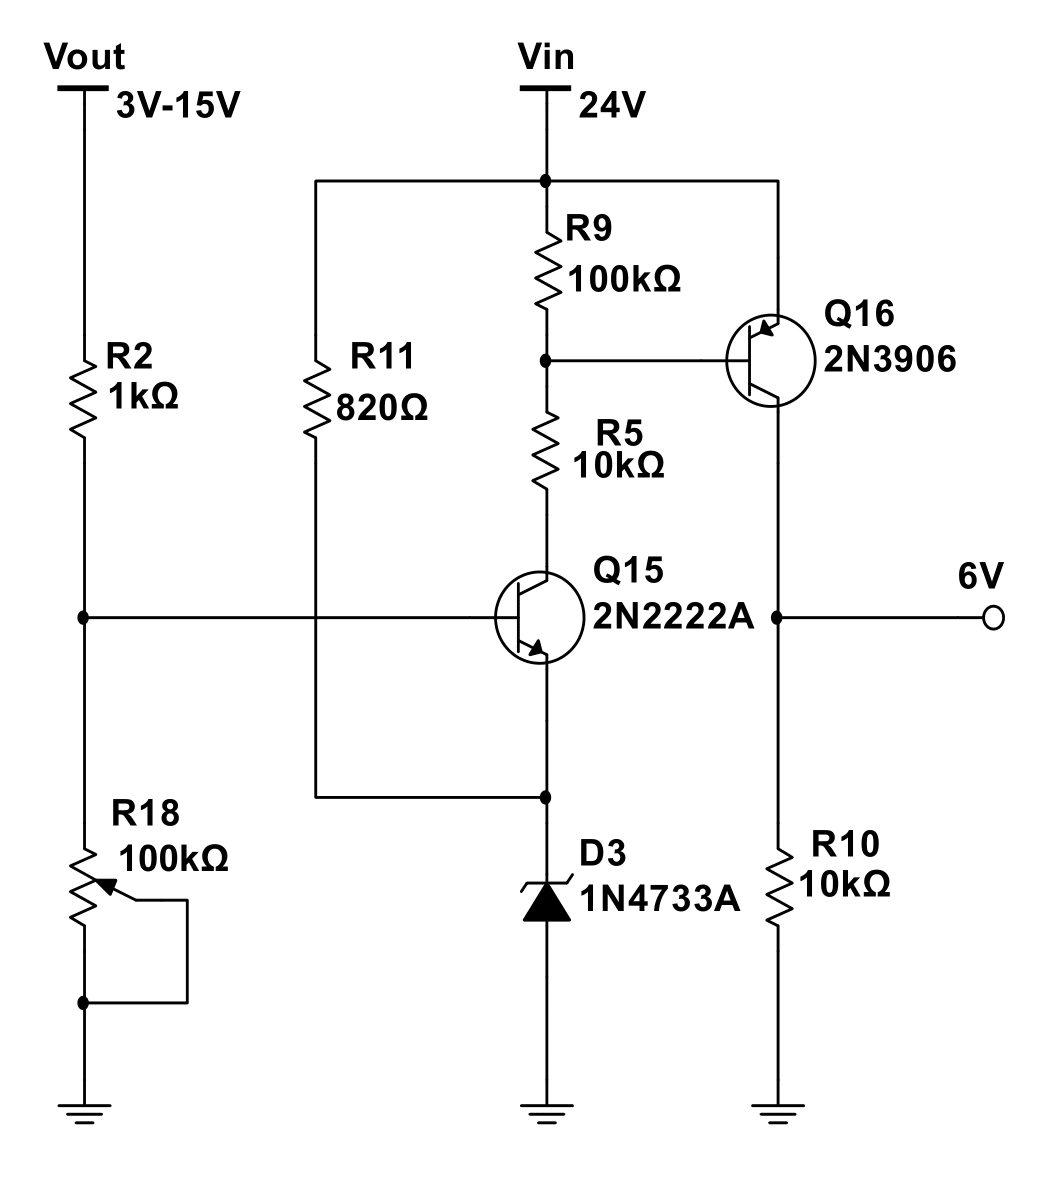
\includegraphics[width=0.6\textwidth]{../imagens/circuito_comparador.png}
    \caption{Circuito final do monitor de tensão}
    \label{fig:monitor_tensao}
\end{figure}

\subsubsection*{Indicador de tensão}

Para indicar a tensão de saída, foram utilizados LEDs de três cores: verde, amarelo e vermelho. Cada LED é acionado conforme a tensão de saída ultrapassa determinados valores, indicando ao usuário as condições de operação do circuito.

Para isso, foi criada uma tabela verdade usando como entrada os sinais digitais gerados pelo comparador de tensão e como saída os LEDs indicadores. Dessa forma, o circuito foi implementado conforme a tabela verdade, garantindo a correta sinalização da tensão de saída.

\begin{table}[htbp]
    \centering
    \caption{Tabela verdade do monitor de tensão}
    \label{tab:exemplo}
    \begin{tabular}{|c|c|c|c|c|}
        \hline
        \textbf{6V} & \textbf{10V} & \textbf{LED VD} & \textbf{LED AM} & \textbf{LED VM} \\
        \hline
        0 & 0 & 1 & 0 & 0 \\
        0 & 1 & 0 & 1 & 0 \\
        1 & 1 & 0 & 0 & 1 \\
        \hline
    \end{tabular}
\end{table}

Dessa forma, foi necessário implementar um circuito lógico que gerasse os sinais de saída conforme a tabela verdade, acionando os LEDs indicadores conforme a tensão de saída do regulador.

\subsubsection*{LED verde}

Para acionar o LED verde, foi utilizado dois transistores NPN ligados um na base do outro, fazendo uma inversão de sinal. O primeiro transistor é acionado quando a tensão de saída é maior que 6 V, acionando o segundo transistor e desligando o LED verde, conforme a tabela verdade. Isso ocorre porque o transistor que está ligado através do seu coletor ao LED verde é polarizado usando um resistor de PULL UP, fazendo com que o LED acenda sempre que o transistor ligado ao sinal de saída do comparador estiver desligado. 

Para a polarização do circuito foram utilizados transistores 2N2222 e resistores de 10 k\(\Omega\). Além disso, foi utilizado um resistor de 1 k\(\Omega\), já calculado anteriormente, para a correta polarização do LED verde. Esse resistor está ligado diretamente ao (\(V_{CC}\)) e ao LED verde, garantindo a correta polarização do LED.

\subsubsection*{LED amarelo}

Para acionar o LED amarelo, foi utilizado a mesma ligação de dois transistores NPN, porém com a diferença de que o primeiro transistor é acionado utilizando o sinal de saída do comparador de 10V e o resistor de polarização do LED amarelo está ligado ao sinal de 6V. Dessa forma, o LED amarelo é acionado quando a tensão de saída está entre 6 V e 10 V, conforme a tabela verdade.

Para a polarização do circuito foram utilizados transistores 2N2222 e resistores de 10 k\(\Omega\). Além disso, foi utilizado um resistor de 1 k\(\Omega\), já calculado anteriormente, para a correta polarização do LED amarelo. 

\subsubsection*{LED vermelho}

Esse LED é o mais fácil de ser implementado, pois ele é acionado quando a tensão de saída é maior que 10 V. Dessa forma, foi utilizado diretamente o sinal proveniente do comparador de 10V para acionar o LED vermelho. Para a correta polarização do LED vermelho, foi utilizado um resistor de 1 k\(\Omega\), já calculado anteriormente.

\subsubsection*{Conclusão do indicador de tensão}

Com os cálculos apresentados, os componentes do indicador de tensão foram dimensionados conforme:

\begin{itemize}
    \item LED verde: 2N2222, 10 k\(\Omega\), 1 k\(\Omega\);
    \item LED amarelo: 2N2222, 10 k\(\Omega\), 1 k\(\Omega\);
    \item LED vermelho: 1 k\(\Omega\).
\end{itemize}

\subsubsection*{Circuito final do indicador de tensão}

O circuito final do indicador de tensão é composto pelos LEDs indicadores, transistores NPN, resistores de polarização, conforme a figura a seguir:

\begin{figure}[H]
    \centering
    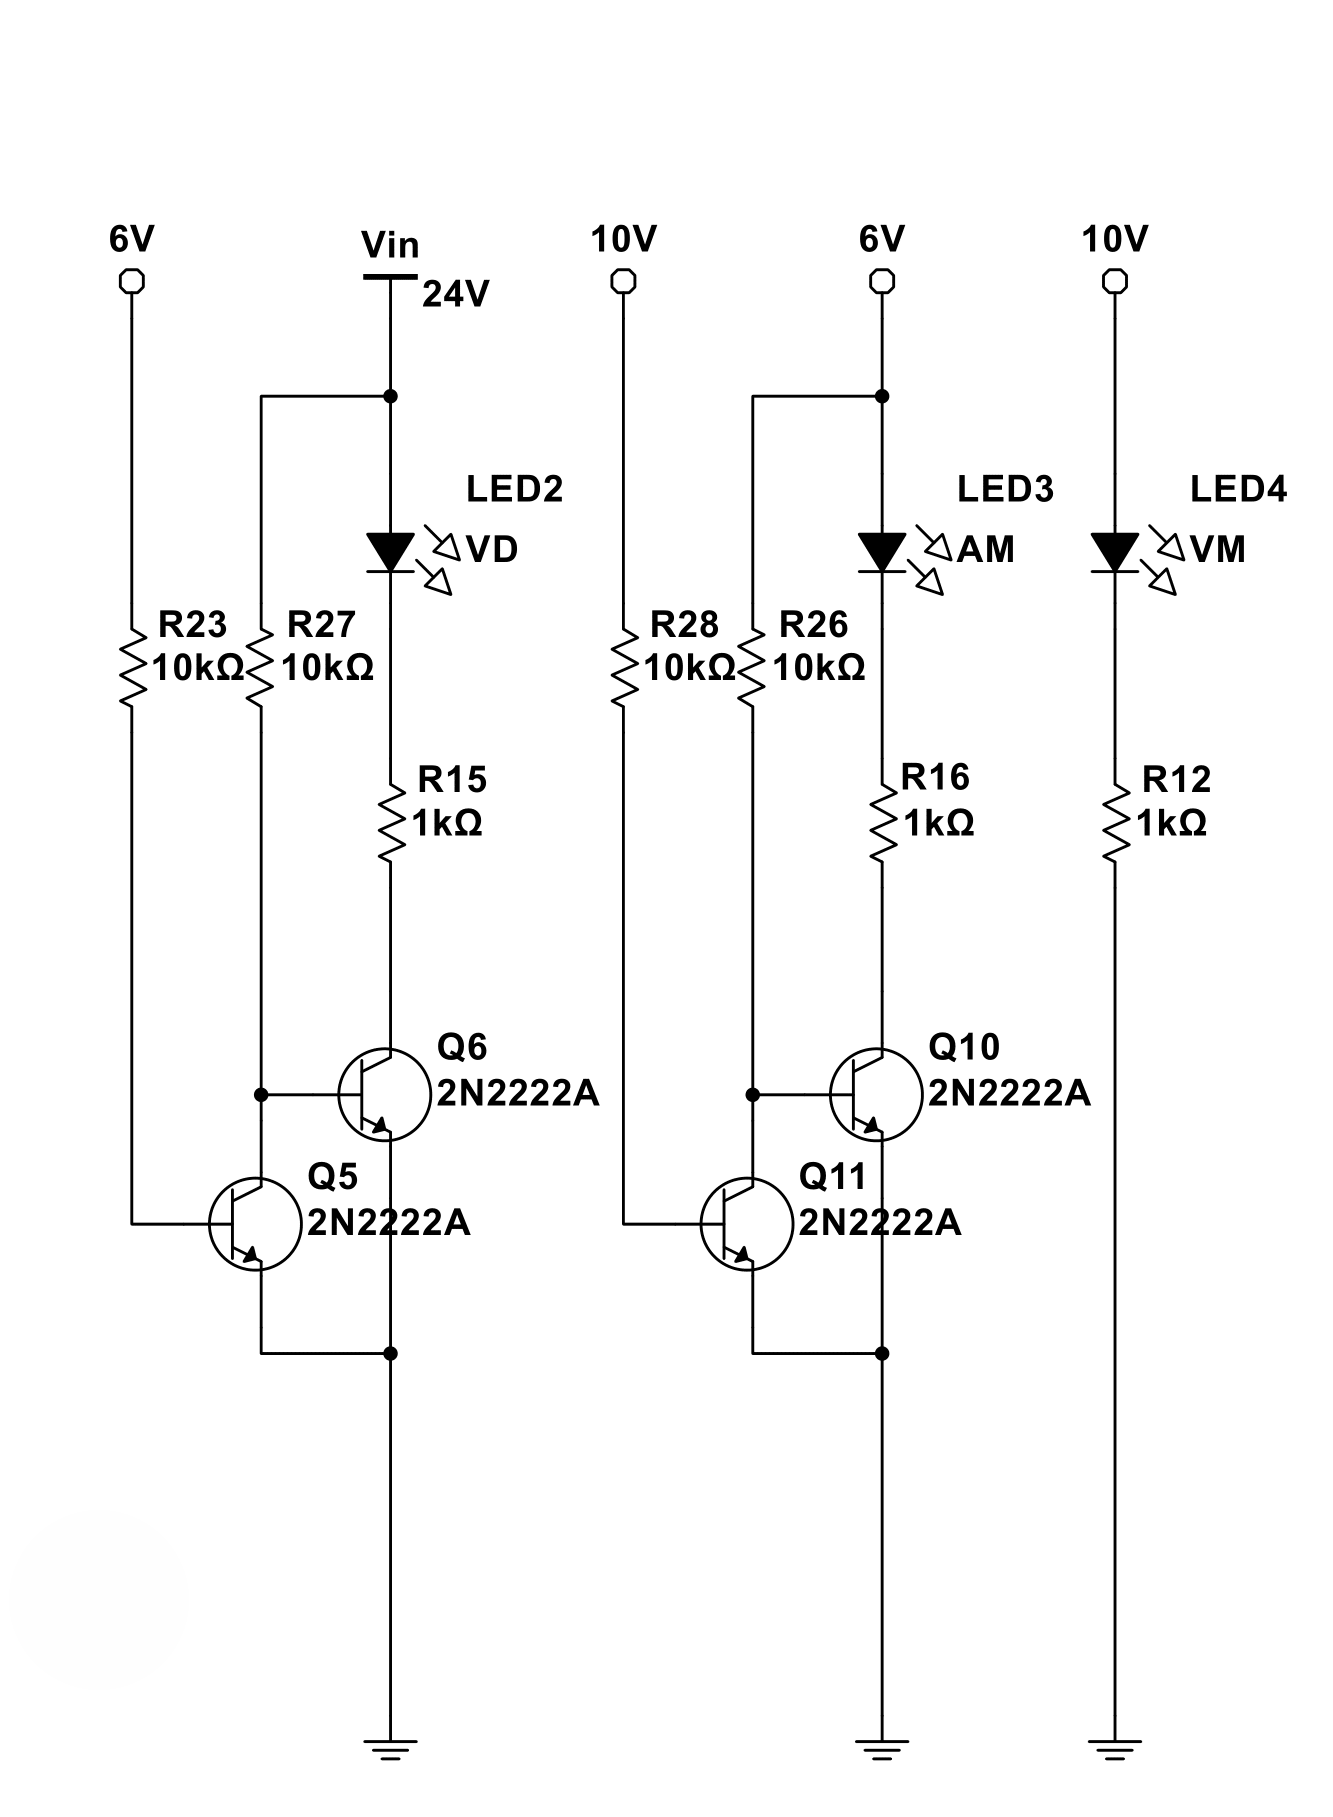
\includegraphics[width=0.6\textwidth]{../imagens/circuito_indicador.png}
    \caption{Circuito final do monitor de tensão}
    \label{fig:indicador_tensao}
\end{figure}

\subsubsection*{Conclusão da fonte linear}

Com todos os cálculos e implementações realizados, a fonte variável foi projetada com sucesso, atendendo a todos os requisitos especificados. O circuito foi implementado com componentes discretos, garantindo a confiabilidade e a precisão do regulador de tensão, do limitador de corrente e da sinalização de tensão. Além disso, a fonte variável foi projetada para fornecer uma tensão ajustável acima do especificado, garantindo a operação segura e confiável do circuito.

\subsubsection*{Circuito final da fonte linear}

O circuito final da fonte variável é composto pelos elementos de regulador de tensão, limitador de corrente, comparador de tensão e indicador de tensão, conforme a figura a seguir:

\begin{figure}[H]
    \centering
    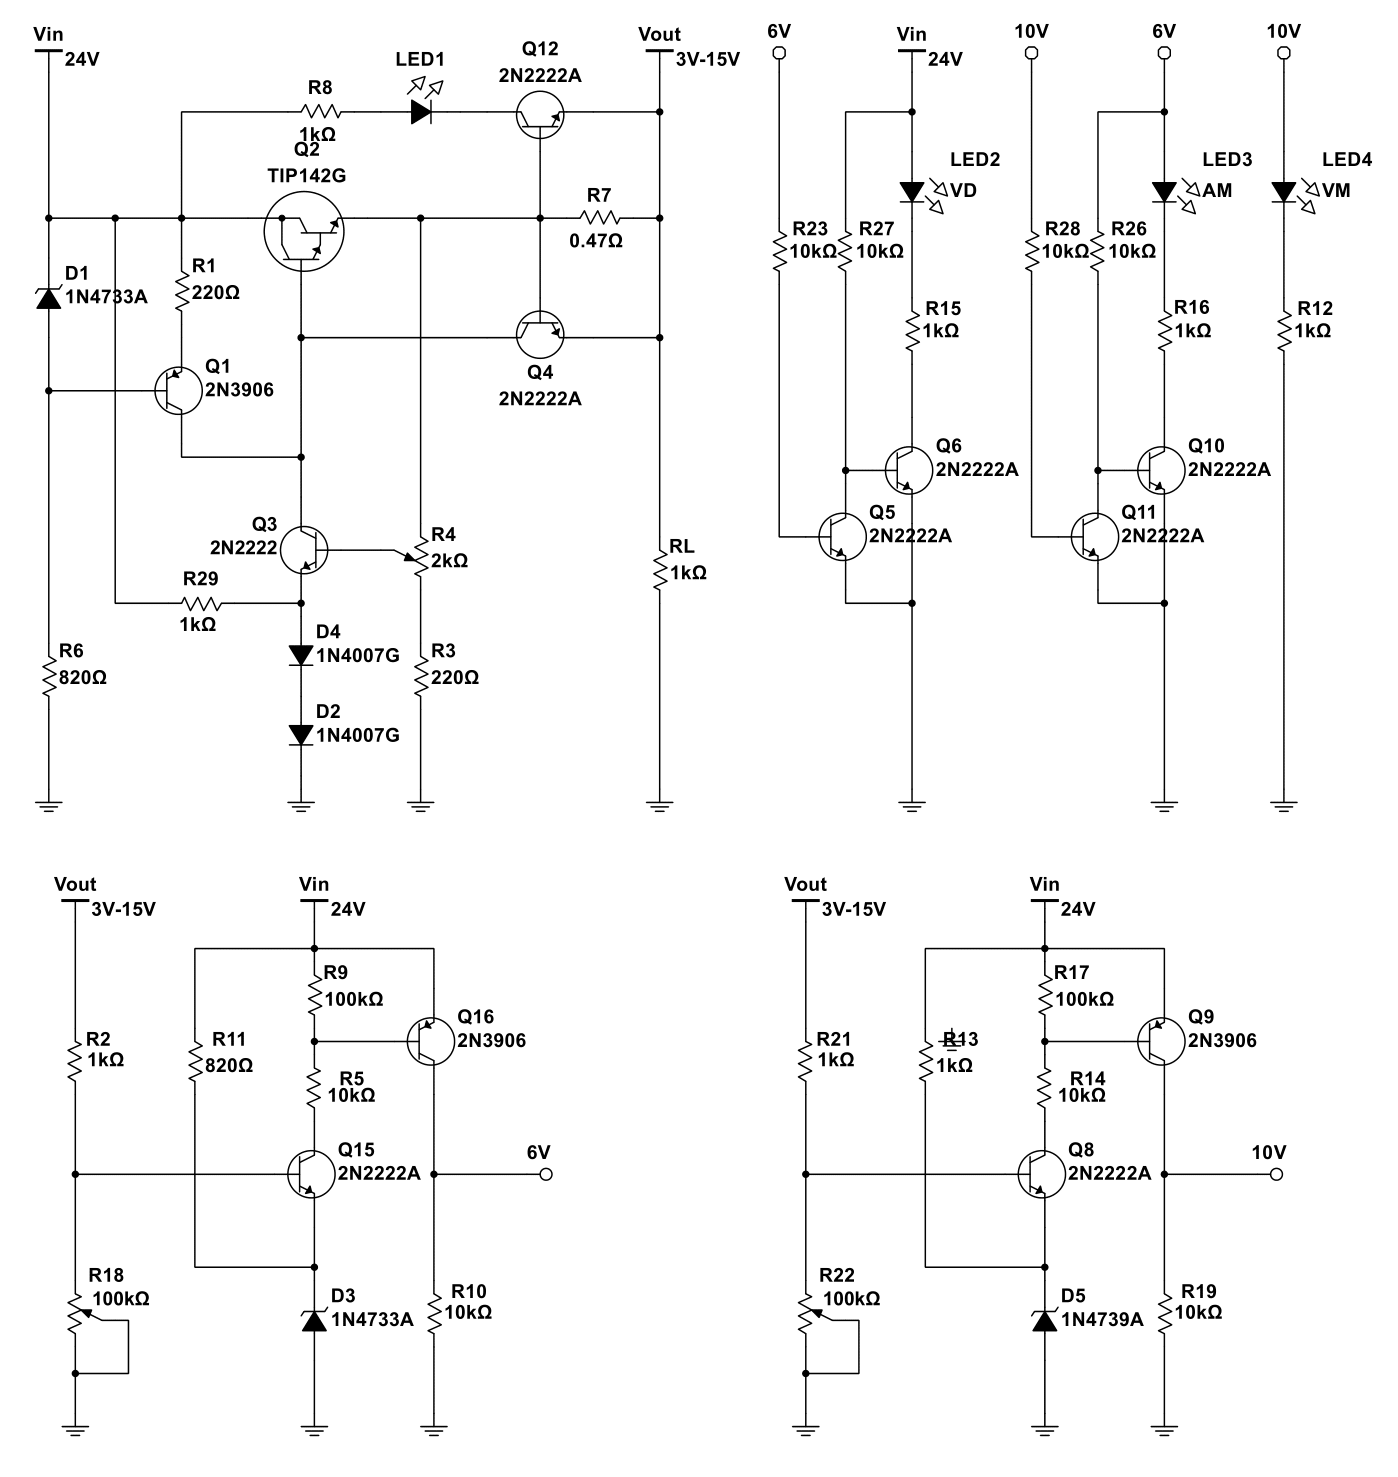
\includegraphics[width=1\textwidth]{../imagens/circuito_final.png}
    \caption{Circuito final da fonte linear}
    \label{fig:final}
\end{figure}

\subsection{Simulação}

O projeto da fonte de alimentação linear com realimentação de tensão foi inicialmente desenvolvido e testado no ambiente de simulação \textit{Multisim® 14.2}, uma ferramenta amplamente utilizada para o estudo e validação de circuitos eletrônicos fornecida pela National Instruments. O uso do simulador permitiu verificar de forma eficiente o desempenho do circuito antes de sua montagem física, reduzindo os riscos de falhas e otimizando o processo de desenvolvimento.

Durante a simulação, foram realizados diversos testes abrangentes para avaliar o comportamento do circuito em diferentes condições de operação. Entre os principais testes realizados destacam-se:

\begin{itemize}
    \item \textbf{Tensão de saída:} Verificação da estabilidade e precisão da tensão de saída em diferentes condições de carga e variações na tensão de entrada.
    \item \textbf{Corrente de saída:} Análise do fornecimento de corrente dentro dos limites especificados, garantindo que o circuito atendesse às exigências de carga.
    \item \textbf{Proteção contra sobrecorrente:} Validação do funcionamento do sistema de proteção, assegurando que o circuito interrompa o fornecimento de corrente em situações de curto-circuito ou excesso de carga.
    \item \textbf{Sinalização de tensão:} Teste das funcionalidades de indicação visual, como LEDs, para informar o estado do circuito (normal, sobrecarga, etc.).
    \item \textbf{Dissipação de potência:} Monitoramento das potências dissipadas nos principais componentes, como transistores, resistores e diodos, para garantir que operem dentro dos limites de segurança térmica especificados pelos fabricantes.
\end{itemize}

A análise detalhada de todos os dispositivos utilizados confirmou a conformidade com os requisitos de projeto, como segurança térmica e confiabilidade dos componentes, assegurando que o circuito é robusto e eficiente.

Notavelmente, o circuito não exigiu ajustes adicionais durante a fase de simulação. Todos os parâmetros de projeto foram atendidos com exatidão, e o circuito se comportou conforme o esperado em todas as condições analisadas. Essa etapa permitiu uma validação inicial eficiente, demonstrando que o circuito era funcional e atendia aos critérios de desempenho estabelecidos, garantindo maior segurança para a etapa de montagem física do protótipo.

\subsection{Montagem}

Após a validação do circuito por meio da simulação, o próximo passo foi a montagem física do protótipo da fonte de alimentação linear. A montagem foi realizada seguindo as diretrizes do projeto, com atenção especial à organização dos componentes, conexões elétricas e segurança do circuito. 

Inicialmente, o grupo realizou a aquisição de todos os componentes necessários para a montagem, garantindo que todos os itens estivessem disponíveis antes do início do processo. Em seguida, os componentes foram organizados e separados de acordo com suas funções, facilitando a montagem e evitando erros durante o processo. 

A montagem foi realizada em um protoboard de alta qualidade, que oferece uma plataforma robusta e confiável para a conexão dos componentes. O uso do protoboard permitiu uma montagem rápida e eficiente, além de facilitar a identificação de possíveis erros e a realização de ajustes durante o processo.

Para uma montagem organizada e segura, o grupo seguiu as seguintes etapas:

\begin{itemize}
    \item \textbf{Instalação dos componentes:} Os componentes foram instalados no protoboard de acordo com o layout do circuito, garantindo que cada item estivesse conectado corretamente e em conformidade com o projeto.
    \item \textbf{Conexões elétricas:} As conexões elétricas foram realizadas com cuidado utilizando fio rígido de 0,5 mm² cortados na medida adequada, garantindo uma conexão sólida e confiável entre os componentes.
    \item \textbf{Testes de continuidade:} Após a montagem, foram realizados testes de continuidade para verificar a integridade das conexões elétricas e garantir que não houvesse interrupções ou falhas no circuito.
    \item \textbf{Verificação visual:} Uma verificação visual foi realizada para garantir que todos os componentes estivessem corretamente instalados e que não houvesse erros evidentes na montagem.
    \item \textbf{Testes preliminares:} Após a montagem, foram realizados testes preliminares para verificar o funcionamento do circuito e identificar possíveis problemas ou erros que precisassem ser corrigidos.
\end{itemize}

Durante o processo de montagem, o grupo adotou uma abordagem cuidadosa e metódica, garantindo que cada etapa fosse concluída com precisão e atenção aos detalhes. A montagem foi realizada de forma colaborativa, com os membros do grupo trabalhando juntos para garantir que o circuito fosse montado corretamente e que todos os componentes estivessem conectados de acordo com o projeto.

Além disso, foi dada atenção especial à organização dos fios e cabos, garantindo que o circuito fosse montado de forma limpa e organizada. Os fios foram cortados na medida adequada e organizados de forma a minimizar a interferência e garantir a integridade das conexões elétricas.

Por fim, um módulo voltímetro amperímetro foi adicionado a fonte de alimentação para monitorar a tensão e corrente de saída do circuito. Esse módulo foi conectado ao circuito de forma a permitir a medição precisa da tensão e corrente fornecida, garantindo o controle e monitoramento eficaz do circuito.

\subsubsection*{Conclusão da montagem}

A montagem do protótipo da fonte de alimentação linear foi concluída com sucesso, atendendo a todos os requisitos de projeto e garantindo o funcionamento correto do circuito. A abordagem cuidadosa e organizada adotada durante o processo de montagem foi fundamental para o sucesso da etapa, garantindo que o circuito fosse montado de forma precisa e confiável.

Após a conclusão da montagem, o grupo realizou testes adicionais para verificar o funcionamento do circuito e garantir que todos os requisitos de projeto fossem atendidos. Os testes incluíram a verificação da tensão de saída, a corrente fornecida, a proteção contra sobrecorrente e a sinalização de tensão, entre outros aspectos.

\subsubsection*{Fotos da montagem}

Na Figura \ref{fig:montagem1}, é possível observar o protótipo da fonte de alimentação linear montado no protoboard, com os componentes organizados e conectados de acordo com o projeto. A montagem foi realizada de forma organizada e cuidadosa, garantindo a integridade do circuito e o correto funcionamento do circuito.

\begin{figure}[H]
    \centering
    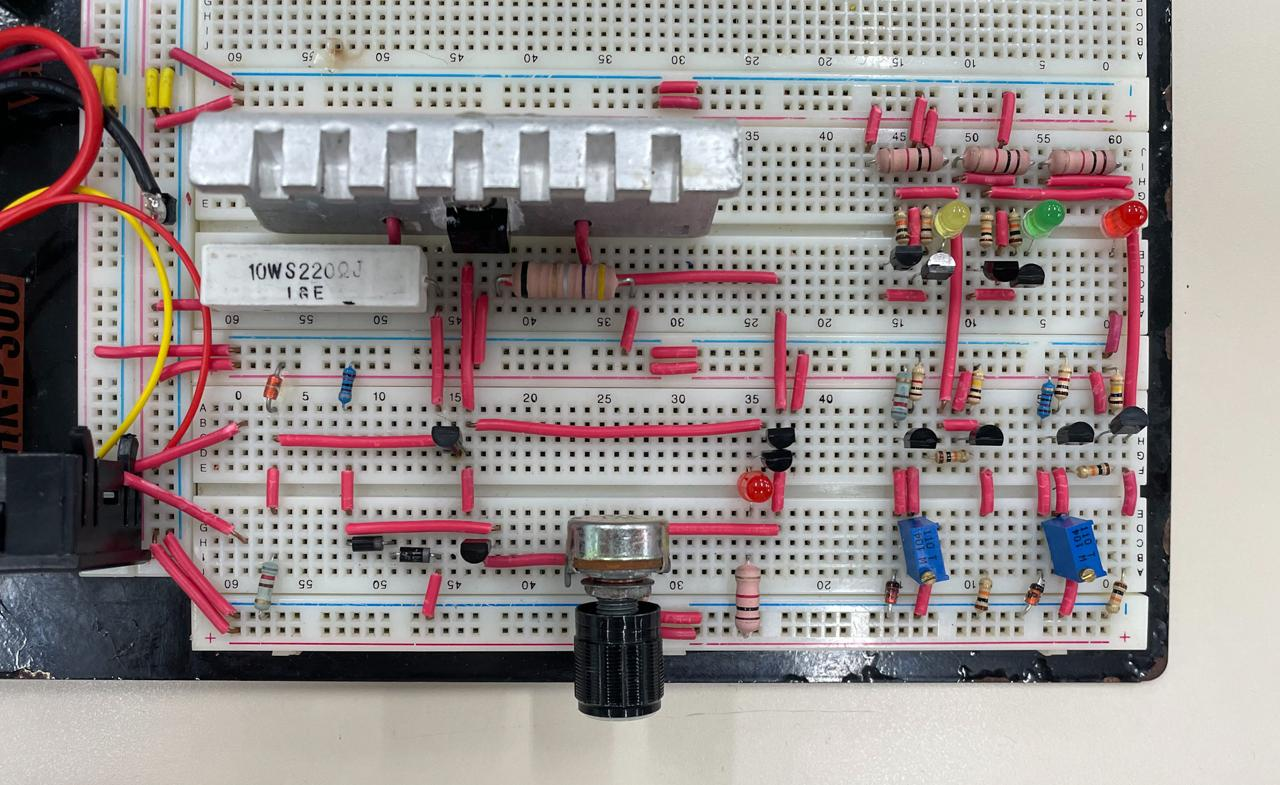
\includegraphics[width=0.6\textwidth]{../imagens/montagem_final.jpg}
    \caption{Montagem do protótipo da fonte de alimentação linear}
    \label{fig:montagem1}
\end{figure}

Na Figura \ref{fig:montagem2}, é possível observar a fonte de alimentação em seu estado de funcionamento de sobre corrente, onde o LED vermelho está aceso, indicando que a corrente de saída ultrapassou o limite de 1 A. Esse estado de funcionamento demonstra a eficácia do sistema de proteção contra sobrecorrente, garantindo a segurança do circuito e dos dispositivos conectados.

\begin{figure}[H]
    \centering
    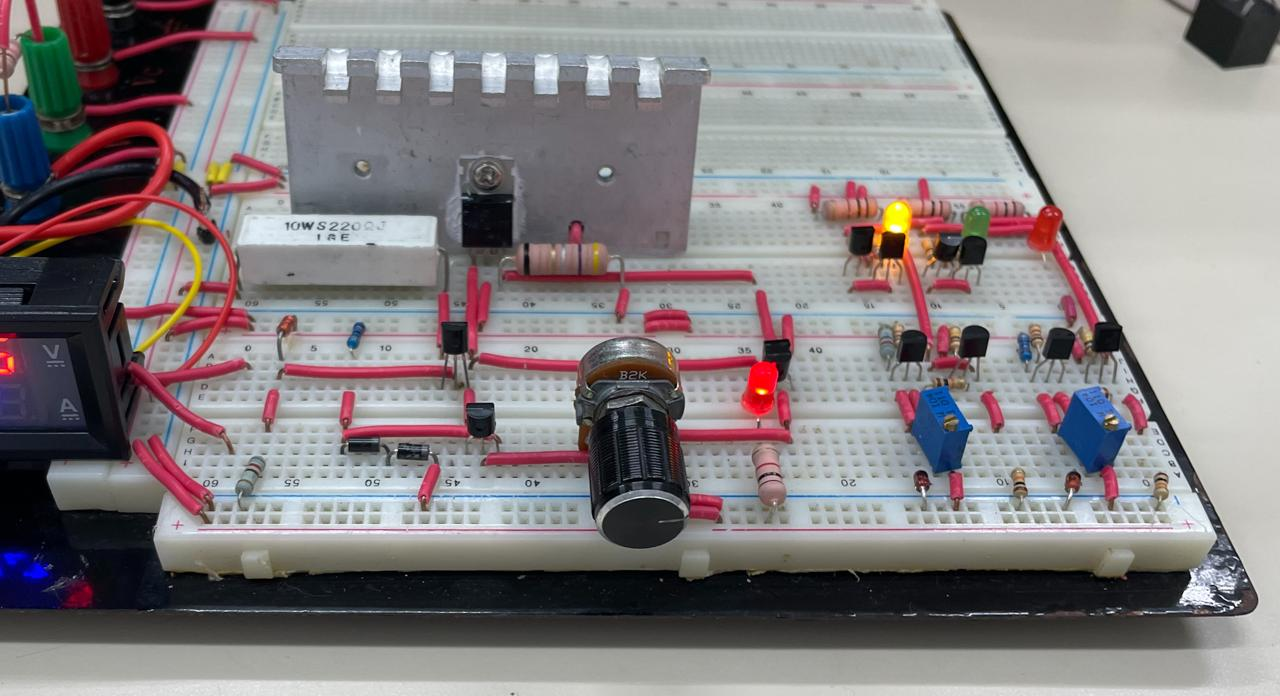
\includegraphics[width=0.6\textwidth]{../imagens/montagem_testes.jpg}
    \caption{Funcionamento da fonte de alimentação em estado de sobre corrente}
    \label{fig:montagem2}
\end{figure}